\documentclass[a4paper,11pt]{article}
\usepackage[T1]{fontenc}
\usepackage[utf8]{inputenc}
\usepackage[english]{babel}
\usepackage{amsmath,amssymb,mathtools}
\usepackage[margin=2.2cm]{geometry}
\usepackage{xcolor,tikz}
\usepackage[most]{tcolorbox}
\setlength{\parindent}{0pt}
\setlength{\parskip}{4pt}
\allowdisplaybreaks
\providecommand{\explainmode}{0}
\newif\ifexplain
\ifnum\explainmode=1 \explaintrue\fi
\newcommand{\aufgabe}[1]{\section*{Exercise #1}}
\newcommand{\angabe}[1]{\textit{#1}\par\smallskip}
\newcommand{\teil}[1]{\subsection*{#1}}
\newcommand{\why}[1]{\text{\small\color{black!65}#1}}
\newtcolorbox{erklbox}{colback=blue!4,colframe=blue!40,breakable,boxrule=0.5pt,title={Erklärung}}
\newcommand{\explain}[1]{\ifexplain\begin{erklbox}#1\end{erklbox}\fi}
\newcommand{\explainfig}[1]{\ifexplain\begin{center}#1\end{center}\fi}
\begin{document}
\begin{center}
{\Large Exercise sheet 3}\\
Linear Optimization (311.160), WS 2026/27\\
Raphael Bleier \qquad 26 October 2026
\end{center}

\explain{Wir schreiben das LP als Gleichungssystem mit nichtnegativen Variablen. Eine Schlupfvariable misst dabei, wie viel bis zur jeweiligen Schranke fehlt. Die Basisvariablen stehen links; die Nichtbasisvariablen wählen wir rechts. Für eine Basislösung setzen wir alle Nichtbasisvariablen auf null. Zulässig ist diese Lösung erst, wenn auch die Basisvariablen nichtnegativ sind. Die Aufteilung und der Variablentausch folgen der Dictionary-Schreibweise aus Lecture 3, Abschnitt 2.2.}

\aufgabe{3.1}
\angabe{Maximize $2x_1+3x_2+x_3$ subject to
\[
x_1+2x_2+x_3+x_4=4,\qquad
2x_1+x_2+2x_3+x_5=5,\qquad x_1,x_2,x_3,x_4,x_5\geq0.
\]
1. Determine $A$ and $b$. 2. Choose a basis and its nonbasis.
3. Write $A_Bx_B=b-A_Nx_N$. 4. Solve for $x_B$ in terms of $x_N$.}

\teil{1. Matrix and right hand side}
With $x=(x_1,x_2,x_3,x_4,x_5)^T$ the system is $Ax=b$, where
\[
\boxed{A=\begin{pmatrix}1&2&1&1&0\\2&1&2&0&1\end{pmatrix},\qquad
b=\begin{pmatrix}4\\5\end{pmatrix}.}
\]
\explain{Jede Zeile steht für eine Nebenbedingung. Die Spalten folgen genau der Reihenfolge im Vektor $x$. Fehlt eine Variable in einer Gleichung, tragen wir dort null ein. Die Zielfunktionskoeffizienten gehören nicht in $A$. Zum Prüfen lesen wir eine Zeile der Matrix noch einmal als Gleichung, weil dabei sowohl eine vertauschte Spalte als auch ein fehlender Koeffizient auffällt, bevor wir mit der Basis weiterrechnen.}
Check by matrix multiplication:
\begin{align*}
Ax&=\begin{pmatrix}1x_1+2x_2+1x_3+1x_4+0x_5\cr2x_1+1x_2+2x_3+0x_4+1x_5\end{pmatrix}&&\why{row times column}\\
&=\begin{pmatrix}x_1+2x_2+x_3+x_4\cr2x_1+x_2+2x_3+x_5\end{pmatrix}&&\why{remove zero terms}
\end{align*}
These are the two given left hand sides.

\teil{2. Basis and nonbasis}
Choose the ordered index sets $B=(4,5)$ and $N=(1,2,3)$. Then
\[
A_B=\begin{pmatrix}1&0\\0&1\end{pmatrix},\quad
A_N=\begin{pmatrix}1&2&1\\2&1&2\end{pmatrix},\quad
x_B=\begin{pmatrix}x_4\\x_5\end{pmatrix},\quad x_N=\begin{pmatrix}x_1\\x_2\\x_3\end{pmatrix}.
\]
\begin{align*}
\det(A_B)&=1\cdot1-0\cdot0&&\why{determinant of a $2\times2$ matrix}\\
&=1-0&&\why{multiply}\\
&=1&&\why{subtract}
\end{align*}
Thus the two selected columns are independent and form a basis.
\[\boxed{B=(4,5),\qquad N=(1,2,3).}\]
\explain{Wir brauchen zwei unabhängige Spalten, weil das System zwei Gleichungen hat. Die Spalten zu $x_4$ und $x_5$ bilden schon die Einheitsmatrix. Damit müssen wir keine weitere Matrix invertieren. Die Reihenfolge behalten wir bei, damit die Einträge von $x_B$ zu den richtigen Spalten gehören. Eine andere Spaltenwahl wäre ebenfalls erlaubt, solange die ausgewählte Teilmatrix invertierbar ist, aber für diese Aufgabe bringt sie keinen Vorteil und macht das Auflösen des Systems nur unnötig länger als nötig.}

\teil{3. Split system}
\begin{align*}
A_Bx_B+A_Nx_N&=b&&\why{partition the columns of $A$}\\
A_Bx_B&=b-A_Nx_N&&\why{subtract $A_Nx_N$}
\end{align*}
\[
\boxed{\begin{pmatrix}1&0\\0&1\end{pmatrix}\begin{pmatrix}x_4\\x_5\end{pmatrix}
=\begin{pmatrix}4\\5\end{pmatrix}-\begin{pmatrix}1&2&1\\2&1&2\end{pmatrix}\begin{pmatrix}x_1\\x_2\\x_3\end{pmatrix}.}
\]
Check: adding $A_Nx_N$ recovers $Ax=b$ with the same column order.
\explain{Hier werden nur die Nichtbasis-Terme nach rechts gebracht. Das Minus gilt für das gesamte Matrixprodukt, nicht bloß für die erste Spalte. Der Inhalt des Gleichungssystems bleibt gleich.}

\teil{4. Solve for the basic variables}
\begin{align*}
x_B&=A_B^{-1}(b-A_Nx_N)&&\why{multiply by $A_B^{-1}$}\\
&=I_2(b-A_Nx_N)&&\why{$A_B$ is the identity}\\
&=b-A_Nx_N&&\why{identity multiplication}\\
&=\begin{pmatrix}4\cr5\end{pmatrix}-\begin{pmatrix}x_1+2x_2+x_3\cr2x_1+x_2+2x_3\end{pmatrix}&&\why{matrix multiplication}\\
&=\begin{pmatrix}4-x_1-2x_2-x_3\cr5-2x_1-x_2-2x_3\end{pmatrix}&&\why{subtract componentwise}
\end{align*}
\[\boxed{x_4=4-x_1-2x_2-x_3,\qquad x_5=5-2x_1-x_2-2x_3.}\]
\explain{Wir können rechts Werte für $x_1,x_2,x_3$ einsetzen und links die beiden übrigen Werte ablesen. Nicht jede Wahl ist zulässig. Auch $x_4$ und $x_5$ müssen mindestens null bleiben. Das unterscheidet eine Lösung der Gleichungen von einer zulässigen Lösung des LP. Wenn eine berechnete Schlupfvariable negativ wird, ist zwar die zugehörige Gleichung weiterhin erfüllt, aber die ursprüngliche obere Schranke wurde überschritten, weshalb wir diesen Punkt trotz korrekter Rechnung nicht verwenden dürfen.}
Check for arbitrary $x_N$:
\begin{align*}
x_1+2x_2+x_3+x_4&=x_1+2x_2+x_3+(4-x_1-2x_2-x_3)&&\why{substitute $x_4$}\\
&=4&&\why{cancel opposite terms}\\
2x_1+x_2+2x_3+x_5&=2x_1+x_2+2x_3+(5-2x_1-x_2-2x_3)&&\why{substitute $x_5$}\\
&=5&&\why{cancel opposite terms}
\end{align*}
The choice must satisfy $x_N\geq0$ and $x_B\geq0$. Setting $x_N=0$ gives
\begin{align*}
x_B&=\begin{pmatrix}4-0-2\cdot0-0\cr5-2\cdot0-0-2\cdot0\end{pmatrix}&&\why{substitute the nonbasic zeros}\\
&=\begin{pmatrix}4\cr5\end{pmatrix}&&\why{evaluate zero terms}
\end{align*}
Both entries are nonnegative, so $(0,0,0,4,5)^T$ is basic feasible.

\aufgabe{3.2}
\angabe{Maximize $z=x_1-2x_2-3x_3$ subject to
\[
-x_1+2x_2+3x_3\leq3,\qquad x_1-x_2-2x_3\leq2,\qquad 2x_1+x_2+x_3\leq7,
\qquad x_1,x_2,x_3\geq0.
\]
1. Introduce $x_4,x_5,x_6$ for standard form and compute the slacks and objective at $x_1=x_2=x_3=0$.
2. Solve for $x_4,x_5,x_6$. How far can only $x_1$ increase while all variables remain nonnegative?
3. Could increasing $x_2$ or $x_3$ help solve the maximization problem?}

\teil{1. Standard form and initial values}
For each upper bound add a nonnegative slack variable:
\[
\boxed{\begin{gathered}
\max\ z=x_1-2x_2-3x_3,\\
-x_1+2x_2+3x_3+x_4=3,\\
x_1-x_2-2x_3+x_5=2,\\
2x_1+x_2+x_3+x_6=7,\\
x_1,x_2,x_3,x_4,x_5,x_6\geq0.
\end{gathered}}
\]
\explain{Bei einer oberen Schranke addieren wir den fehlenden Rest zur linken Seite. Deshalb steht vor jeder Schlupfvariable ein Plus. Die Forderung $x_4,x_5,x_6\geq0$ stellt sicher, dass die ursprüngliche Schranke nicht überschritten wird. Die Zielfunktion ändert sich dadurch nicht.}
At the origin:
\begin{align*}
-0+2\cdot0+3\cdot0+x_4&=3&&\why{substitute $x_1,x_2,x_3$}\\
x_4&=3&&\why{evaluate zero terms}\\
0-0-2\cdot0+x_5&=2&&\why{substitute $x_1,x_2,x_3$}\\
x_5&=2&&\why{evaluate zero terms}\\
2\cdot0+0+0+x_6&=7&&\why{substitute $x_1,x_2,x_3$}\\
x_6&=7&&\why{evaluate zero terms}\\
z&=0-2\cdot0-3\cdot0&&\why{substitute in the objective}\\
&=0&&\why{evaluate zero terms}
\end{align*}
\[\boxed{(x_4,x_5,x_6)=(3,2,7),\qquad z=0.}\]
Check: the original three left hand sides are zero at the origin, hence satisfy their positive upper bounds.

\teil{2. Initial dictionary and increase of $x_1$}
\begin{align*}
-x_1+2x_2+3x_3+x_4&=3&&\why{first equation}\\
2x_2+3x_3+x_4&=3+x_1&&\why{add $x_1$}\\
3x_3+x_4&=3+x_1-2x_2&&\why{subtract $2x_2$}\\
x_4&=3+x_1-2x_2-3x_3&&\why{subtract $3x_3$}
\end{align*}
\explain{Das Minus vor $x_1$ in der ursprünglichen Nebenbedingung wird beim Verschieben zum Plus. Wenn nur $x_1$ steigt, wächst also $x_4$. Diese erste Zeile begrenzt den Schritt nach oben nicht.}
\begin{align*}
x_1-x_2-2x_3+x_5&=2&&\why{second equation}\\
-x_2-2x_3+x_5&=2-x_1&&\why{subtract $x_1$}\\
-2x_3+x_5&=2-x_1+x_2&&\why{add $x_2$}\\
x_5&=2-x_1+x_2+2x_3&&\why{add $2x_3$}
\end{align*}
\begin{align*}
2x_1+x_2+x_3+x_6&=7&&\why{third equation}\\
x_2+x_3+x_6&=7-2x_1&&\why{subtract $2x_1$}\\
x_3+x_6&=7-2x_1-x_2&&\why{subtract $x_2$}\\
x_6&=7-2x_1-x_2-x_3&&\why{subtract $x_3$}
\end{align*}
\[\boxed{x_4=3+x_1-2x_2-3x_3,\quad x_5=2-x_1+x_2+2x_3,\quad x_6=7-2x_1-x_2-x_3.}\]
Keep $x_2=x_3=0$ and set $x_1=t\geq0$:
\begin{align*}
x_4&=3+t-2\cdot0-3\cdot0&&\why{substitute}\\
&=3+t&&\why{evaluate zero terms}\\
x_5&=2-t+0+2\cdot0&&\why{substitute}\\
&=2-t&&\why{evaluate zero terms}\\
x_6&=7-2t-0-0&&\why{substitute}\\
&=7-2t&&\why{evaluate zero terms}
\end{align*}
\explain{Jetzt ändern wir wirklich nur eine Variable. Für jede Basisvariable prüfen wir, ab welchem Wert von $t$ sie null wird. Die erste solche Schranke beendet den zulässigen Schritt. Das ist der Minimum-Ratio-Test aus der Vorlesung. Wir dürfen nicht die größere der beiden oberen Grenzen wählen, weil zu diesem Zeitpunkt die kleinere Grenze schon überschritten wäre und damit mindestens eine Basisvariable einen negativen Wert angenommen hätte.}
The first slack is nonnegative for every $t\geq0$. For the other two:
\begin{align*}
2-t&\geq0&&\why{nonnegativity of $x_5$}\\
2&\geq t&&\why{add $t$}\\
7-2t&\geq0&&\why{nonnegativity of $x_6$}\\
7&\geq2t&&\why{add $2t$}\\
\frac72&\geq t&&\why{divide by positive $2$}
\end{align*}
\[\boxed{0\leq x_1\leq2;\qquad x_1\text{ can increase by }2,\text{ and }x_5\text{ leaves the basis}.}\]
At the endpoint:
\begin{align*}
x_4&=3+2&&\why{substitute $t=2$}\\
&=5&&\why{add}\\
x_5&=2-2&&\why{substitute $t=2$}\\
&=0&&\why{subtract}\\
x_6&=7-2\cdot2&&\why{substitute $t=2$}\\
&=7-4&&\why{multiply}\\
&=3&&\why{subtract}
\end{align*}
Check in the original inequalities:
\begin{align*}
-x_1+2x_2+3x_3&=-2+2\cdot0+3\cdot0&&\why{substitute $(2,0,0)$}\\
&=-2&&\why{evaluate zero terms}\\
-2&\leq3&&\why{first bound}\\
x_1-x_2-2x_3&=2-0-2\cdot0&&\why{substitute}\\
&=2&&\why{evaluate zero terms}\\
2&\leq2&&\why{second bound}\\
2x_1+x_2+x_3&=2\cdot2+0+0&&\why{substitute}\\
&=4&&\why{multiply and remove zeros}\\
4&\leq7&&\why{third bound}
\end{align*}

\teil{3. Other entering variables}
At the initial basic solution, increasing only $x_2=t$ gives
\begin{align*}
z&=0-2t-3\cdot0&&\why{set $x_1$ and $x_3$ to zero}\\
&=-2t&&\why{remove zeros}\\
z&<0&&\why{$t$ positive}
\end{align*}
Increasing only $x_3=t$ instead gives
\begin{align*}
z&=0-2\cdot0-3t&&\why{set $x_1$ and $x_2$ to zero}\\
&=-3t&&\why{remove zeros}\\
z&<0&&\why{$t$ positive}
\end{align*}
\[\boxed{\text{Neither }x_2\text{ nor }x_3\text{ gives an improving initial step}.}\]
Check: both slopes, $-2$ and $-3$, are strictly negative, whereas the initial objective is zero.
\explain{Eine zulässige Bewegung ist noch keine Verbesserung. Beide Variablen könnten zunächst ein Stück wachsen, aber der Zielfunktionswert sinkt dabei. Für das Maximum wählen wir hier $x_1$ mit positivem Koeffizienten. Diese Aussage betrifft den einzelnen Schritt ab der Startlösung, nicht beliebige gleichzeitige Änderungen mehrerer Variablen.}

\aufgabe{3.3}
\angabe{Continue with Exercise 3.2. 4. Express $x_1,x_4,x_6$ in terms of $x_2,x_3,x_5$.
5. Express the objective in these variables and explain why the current basic solution is optimal.
6. State the optimal solution and optimal objective value.}

\teil{4. New dictionary}
Solve the second equation for the new basic variable $x_1$:
\begin{align*}
x_5&=2-x_1+x_2+2x_3&&\why{previous dictionary}\\
x_1+x_5&=2+x_2+2x_3&&\why{add $x_1$}\\
x_1&=2+x_2+2x_3-x_5&&\why{subtract $x_5$}
\end{align*}
\explain{Wir tauschen $x_1$ und $x_5$. Das heißt Pivot: $x_1$ wird Basisvariable, $x_5$ Nichtbasisvariable. Die neue Gleichung setzen wir in die anderen Basiszeilen und in die Zielfunktion ein. Dabei dürfen keine alten Basisvariablen rechts übrig bleiben.}
\begin{align*}
x_4&=3+x_1-2x_2-3x_3&&\why{previous dictionary}\\
&=3+(2+x_2+2x_3-x_5)-2x_2-3x_3&&\why{substitute $x_1$}\\
&=(3+2)+(1-2)x_2+(2-3)x_3-x_5&&\why{collect equal terms}\\
&=5-x_2-x_3-x_5&&\why{evaluate coefficients}
\end{align*}
\explain{In der ersten Zeile wird $x_1$ mit Faktor $+1$ ersetzt. Die neuen Koeffizienten von $x_2$ und $x_3$ sind deshalb jeweils $-1$. Die Konstante steigt von $3$ auf $5$.}
\begin{align*}
x_6&=7-2x_1-x_2-x_3&&\why{previous dictionary}\\
&=7-2(2+x_2+2x_3-x_5)-x_2-x_3&&\why{substitute $x_1$}\\
&=7-4-2x_2-4x_3+2x_5-x_2-x_3&&\why{distribute $-2$}\\
&=(7-4)+(-2-1)x_2+(-4-1)x_3+2x_5&&\why{collect equal terms}\\
&=3-3x_2-5x_3+2x_5&&\why{evaluate coefficients}
\end{align*}
\explain{Hier steht vor der Klammer $-2$. Dieser Faktor trifft jeden Term. Besonders beim letzten Term ist das Vorzeichen wichtig: Aus $-2(-x_5)$ wird $+2x_5$.}
\[\boxed{\begin{aligned}
x_1&=2+x_2+2x_3-x_5,\\
x_4&=5-x_2-x_3-x_5,\\
x_6&=3-3x_2-5x_3+2x_5.
\end{aligned}}\]
The new basis is $B=(1,4,6)$ and the nonbasis is $N=(2,3,5)$.
Check the identities in all three original equations:
\begingroup\small
\begin{align*}
-x_1+2x_2+3x_3+x_4&=-(2+x_2+2x_3-x_5)+2x_2+3x_3+(5-x_2-x_3-x_5)&&\why{substitute}\\
&=-2-x_2-2x_3+x_5+2x_2+3x_3+5-x_2-x_3-x_5&&\why{remove parentheses}\\
&=(-2+5)+(-1+2-1)x_2+(-2+3-1)x_3+(1-1)x_5&&\why{collect terms}\\
&=3&&\why{evaluate coefficients}\\
x_1-x_2-2x_3+x_5&=(2+x_2+2x_3-x_5)-x_2-2x_3+x_5&&\why{substitute}\\
&=2&&\why{cancel opposite terms}\\
2x_1+x_2+x_3+x_6&=2(2+x_2+2x_3-x_5)+x_2+x_3+(3-3x_2-5x_3+2x_5)&&\why{substitute}\\
&=4+2x_2+4x_3-2x_5+x_2+x_3+3-3x_2-5x_3+2x_5&&\why{distribute $2$}\\
&=(4+3)+(2+1-3)x_2+(4+1-5)x_3+(-2+2)x_5&&\why{collect terms}\\
&=7&&\why{evaluate coefficients}
\end{align*}
\endgroup

\teil{5. Objective and optimality}
\begin{align*}
z&=x_1-2x_2-3x_3&&\why{original objective}\\
&=(2+x_2+2x_3-x_5)-2x_2-3x_3&&\why{substitute $x_1$}\\
&=2+(1-2)x_2+(2-3)x_3-x_5&&\why{collect terms}\\
&=2-x_2-x_3-x_5&&\why{evaluate coefficients}\\
z&\leq2&&\why{all nonbasic variables nonnegative}
\end{align*}
At $x_2=x_3=x_5=0$ the dictionary gives:
\begin{align*}
x_1&=2+0+2\cdot0-0&&\why{substitute}\\
&=2&&\why{evaluate zeros}\\
x_4&=5-0-0-0&&\why{substitute}\\
&=5&&\why{evaluate zeros}\\
x_6&=3-3\cdot0-5\cdot0+2\cdot0&&\why{substitute}\\
&=3&&\why{evaluate zeros}\\
z&=2-0-0-0&&\why{substitute}\\
&=2&&\why{evaluate zeros}
\end{align*}
All basic values are nonnegative. The upper bound is attained, so this basic solution is optimal. $\square$
\[\boxed{z=2-x_2-x_3-x_5\leq2,\qquad z^*=2.}\]
\explain{Die Koeffizienten der Nichtbasisvariablen in dieser Zielfunktionszeile heißen reduzierte Kosten. Alle drei sind negativ. Weil die Variablen nichtnegativ sind, kann kein zulässiger Punkt mehr als $2$ erreichen. Unsere Basislösung erreicht genau diesen Wert. Das ist eine globale Schranke und beweist daher mehr als nur das Fehlen eines besseren einzelnen Schritts. Entscheidend ist, dass wir dieselbe Zielfunktion durch Einsetzen nur anders geschrieben haben, sodass diese Schranke für sämtliche zulässigen Lösungen gilt und nicht bloß für die gerade untersuchte Bewegung entlang einer Kante.}

\teil{6. Optimal solution and check}
\[\boxed{(x_1^*,x_2^*,x_3^*)=(2,0,0),\qquad (x_4^*,x_5^*,x_6^*)=(5,0,3),\qquad z^*=2.}\]
The full standard-form solution is $(2,0,0,5,0,3)^T$. Check:
\begin{align*}
-x_1+2x_2+3x_3+x_4&=-2+2\cdot0+3\cdot0+5&&\why{substitute}\\
&=-2+5&&\why{evaluate zero terms}\\
&=3&&\why{add}\\
x_1-x_2-2x_3+x_5&=2-0-2\cdot0+0&&\why{substitute}\\
&=2&&\why{evaluate zero terms}\\
2x_1+x_2+x_3+x_6&=2\cdot2+0+0+3&&\why{substitute}\\
&=4+3&&\why{multiply and remove zeros}\\
&=7&&\why{add}\\
z&=2-2\cdot0-3\cdot0&&\why{substitute in original objective}\\
&=2&&\why{evaluate zero terms}
\end{align*}
All six variables are nonnegative. Equality in the upper bound requires $x_2+x_3+x_5=0$.
Since the three terms are nonnegative, each must be zero. The dictionary then fixes $x_1=2$, so the optimal solution is unique. $\square$
\explain{In der ursprünglichen Aufgabe werden nur die ersten drei Variablen gesucht. Die Schlupfwerte dienen zusätzlich als Kontrolle. Die zweite Nebenbedingung ist aktiv, weil $x_5$ null ist. Bei der ersten bleiben $5$ Einheiten frei, bei der dritten $3$. Auch die Eindeutigkeit lässt sich direkt aus der Zielfunktionszeile lesen: Für denselben Optimalwert darf keiner der drei abgezogenen Terme positiv sein.}

\explainfig{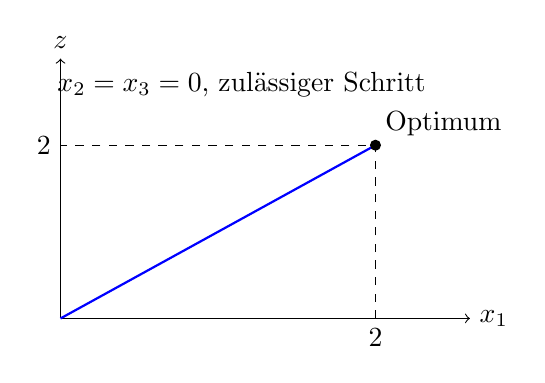
\begin{tikzpicture}[x=2cm,y=1.1cm]
\draw[->] (0,0)--(2.6,0) node[right] {$x_1$};
\draw[->] (0,0)--(0,3) node[above] {$z$};
\draw[thick,blue] (0,0)--(2,2);
\draw[dashed] (2,0)--(2,2)--(0,2);
\fill (2,2) circle (2pt) node[above right] {Optimum};
\node[below] at (2,0) {$2$}; \node[left] at (0,2) {$2$};
\node at (1.15,2.7) {$x_2=x_3=0$, zulässiger Schritt};
\end{tikzpicture}}

\explain{Classroom task 3.1 ist laut Workflow nicht Teil der schriftlichen Abgabe. Als Lernzusatz: Gesucht ist die zulässige Menge von $x_1+x_2\leq2$, $x_2\leq1$, $x_1,x_2\geq0$ bei Zielfunktion $x_1+2x_2$. Ihre Ecken sind $(0,0)$, $(2,0)$, $(1,1)$ und $(0,1)$.
Mit Schlupfvariablen stehen die Gleichungen $x_1+x_2+x_3=2$ und $x_2+x_4=1$. Aus der zweiten isolieren wir $x_2=1-x_4$. Einsetzen in die erste liefert $x_1+(1-x_4)+x_3=2$. Wir ziehen die Klammer ab und erhalten $x_1=2-(1-x_4)-x_3$. Ausmultiplizieren liefert $x_1=2-1+x_4-x_3$, also $x_1=1+x_4-x_3$.
Für $x_3=x_4=0$ ist $x_2=1-0=1$ und $x_1=1+0-0=1$. Die Probe lautet $1+1=2$ und $1\leq1$; beide Koordinaten sind nichtnegativ. Die Basislösung ist also zulässig. Das gesuchte Wort ist \emph{vertices} (Eckpunkte).}
\explainfig{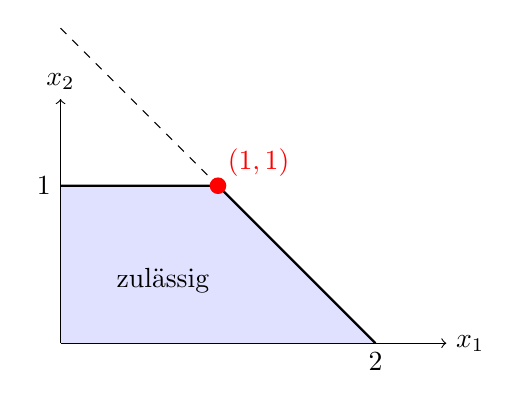
\begin{tikzpicture}[scale=2]
\fill[blue!12] (0,0)--(2,0)--(1,1)--(0,1)--cycle;
\draw[->] (0,0)--(2.45,0) node[right] {$x_1$};
\draw[->] (0,0)--(0,1.55) node[above] {$x_2$};
\draw[thick] (0,1)--(1,1)--(2,0);
\draw[dashed] (0,2)--(2,0);
\fill[red] (1,1) circle (1.5pt) node[above right] {$(1,1)$};
\node[below] at (2,0) {$2$}; \node[left] at (0,1) {$1$};
\node at (0.65,0.4) {zulässig};
\end{tikzpicture}}
\end{document}
